\documentclass[11pt]{article}
\usepackage{amssymb}
\usepackage{amsmath}
\usepackage{physics}
\usepackage{xcolor}
\usepackage[left=3.6cm,right=3.9cm,top=2.5cm,bottom=2cm,bindingoffset=0cm]{geometry}
\usepackage{graphicx}
\begin{document}

\begin{flushright}
B0B33OPT\\
Karina Balagazova
\end{flushright}
\part*{NLLS: Kružnice}

\section{Proložení bodů kružnicí}


\subsection{dist(x, a)}
\paragraph{}
Máme $a_{1},...,a_{m} \in \mathbb{R}^{2}$. Označme jako $x = (c, r) \in \mathbb{R}^{3}$ vektor parametrů kružnice. Funkce $dist(x, a)$ je orientovaná vzdálenost bodu $a$ od kružnice s parametry $x$. Spočitáme ji jako
$$ dist(x, a) = \|c-a_{i}\| - r$$
přičemž pro $a$ vně kružnice je $ dist(x, a) > 0 $ a pro $a$ uvnitř kružnice je $ dist(x, a) < 0$.

Jacobiho matice této funkce bude vypadat takto: 
$$ dist'(x, a) = 
\begin{bmatrix}
\dfrac{c_{1} - a_{i_{1}}}{\|c-a_{i}\|} & \dfrac{c_{2} - a_{i_{2}}}{\|c-a_{i}\|} & -1
\end{bmatrix}$$


\subsection{Gauss-Newtonova metoda}
Iterační krok: 
$$\mathbf{x_{new} = x - (g'(x)^{T} g'(x))^{-1} g'(x)^{T}g(x)}$$

\subsection{Levenberg-Marquardtova metoda}
Iterační krok: 
$$\mathbf{x_{new} = x - (g'(x)^{T} g'(x) + \mu_{k}I)^{-1} g'(x)^{T}g(x)}$$




\section*{Úkoly}

\subsection*{1 Diferencovatelnost funkce $f$}
$$f(x) = \sum_{i = 1}^{m} dist(x, a_{i})^{2} = \|dist(x, a)\|^{2}$$
Postačující podmínkou pro diferencovatelnost funkce v bodě $x$ je existence a spojitost všech parciálních derivací funkce v tomto bodě. Zkusíme tedy funkci $f$ zderivovat
$$ f'(x) = 2 dist(x, a)^{T} dist'(x, a)$$
Pro existenci $dist'(x, a)$ musí platit nasledující: 
$$ \|c-a_{i}\| \neq 0$$ tj. funkce $f$ je diferencovatelná tehdy, když $c \neq a_{i}$. Jinými slovy střed kružnice by neměl ležet v žádném z bodů $a_{1},...,a_{m}$.


\subsection*{2 Omezení $r \geq 0$}
\paragraph{}
Ignorování této podmínky by nemělo nic změnit. Během prvních iterací funkce $f$  bude nabývat větších hodnot, než by nabývala s kladným $r$.  Pak se ale situace změní a znaménko se stane kladným, protože vždycky bude existovat lepší kladné $r$, ke kterému pak bude metoda konvergovat.


\subsection*{3 Lokální minima s různou funkční hodnotou}
\paragraph{}
Nejdříve musíme zvolit vhodný počet bodů. Například pro $ m = 2 $ (tj. libovolné dva body), funkční hodnota všech lokálních minim vždy zkonverguje k nule. Proto zvolíme větší $m$.

Zkusíme spustit Gauss-Newtonovou metodu pro body $a_{1},...,a_{5}$ a počáteční odhady $x_{0_{1}}$ a $x_{0_{2}}$:
$$a = 
\begin{bmatrix}
0 & -0.5 & 0.5 & -0.6 & 0.6\\
0 & -0.5 &-0.5 & 0.5 & 0.5
\end{bmatrix}, 
x_{0_{1}} = 
\begin{bmatrix}
0\\
0.5\\
0.7
\end{bmatrix},
x_{0_{2}} = 
\begin{bmatrix}
0\\
-0.5\\
0.7
\end{bmatrix}
$$
Metoda zkonverguje do dvou různých stacionárních bodů, a vzhledem k tomu, že jsme použili Gauss-Newtonovou metodu, tak téměř jistě víme, že jsou to lokální minima. Po 20 iterací dostaneme parametry: 
$$x_{1} = 
\begin{bmatrix}
0.0000\\
-0.1818\\
0.6367\\
\end{bmatrix},
x_{2} = 
\begin{bmatrix}
0.0000\\
0.2601\\
0.6744\\
\end{bmatrix}
$$

$$ f(x_{1}) = 0.2841, f(x_{2}) = 0.3583$$

$$ \nabla f(x_{1}) =
\begin{bmatrix}
0.0134\\
0.2220\\
-0.7772
\end{bmatrix},
\nabla f(x_{2}) = 
\begin{bmatrix}
-0.0073\\
0.4441\\
0.2220
\end{bmatrix}$$

\begin{figure}[h]
    
    \begin{minipage}{0.45\textwidth}
        
        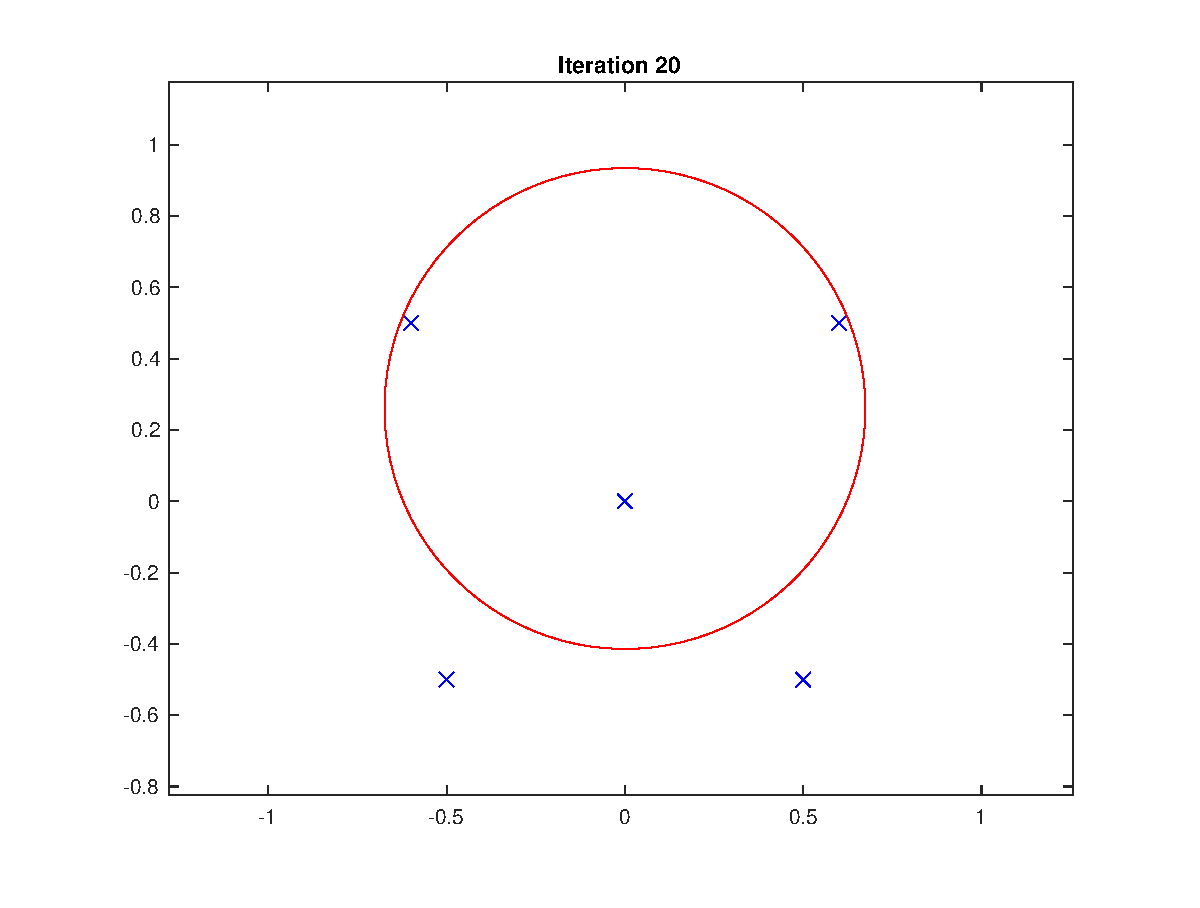
\includegraphics[width=9cm]{circle1.eps}
    \end{minipage}\hfill
    \hspace{.05\linewidth}
    \begin{minipage}{0.45\textwidth}
        \centering
        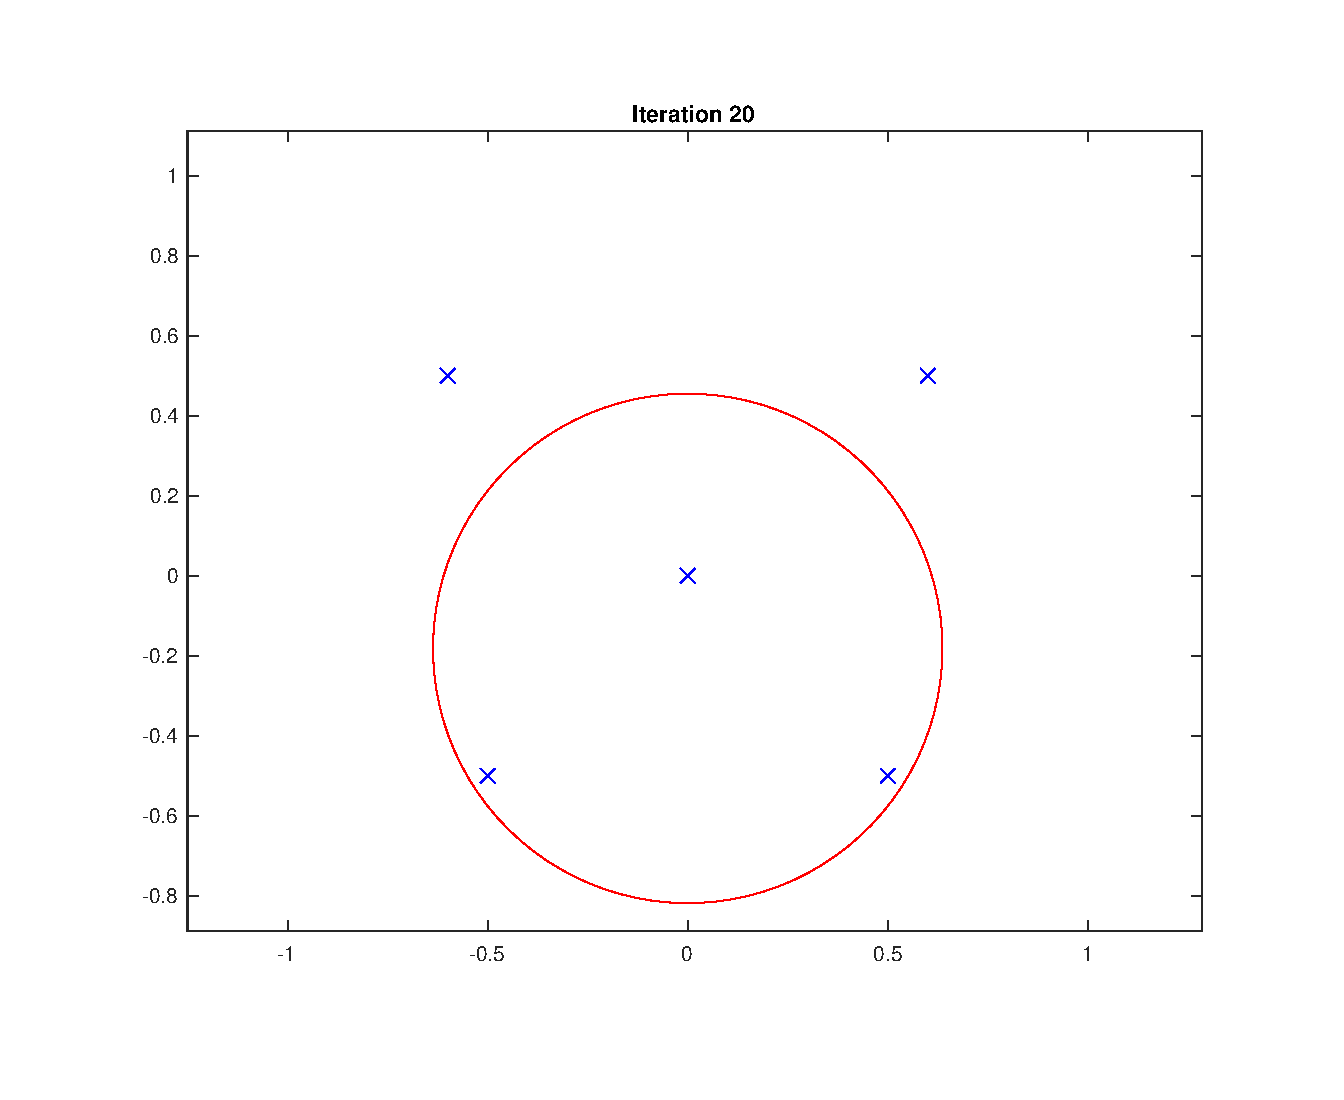
\includegraphics[width=9cm]{circle2.eps}
    \end{minipage}
\end{figure}

\subsection*{4 Minimalizace funkce přes dvě proměnné}
\paragraph{}

Abychom mohli najít minimum funkce, její derivace v tomto bodě musí být 0:
$$ \pdv{f}{r} = 2 \sum_{i = 1}^{m} dist(x, a_{i})* (-1) = -2 \sum_{i = 1}^{m} (\|c-a_{i}\| - r) = 0$$
$$ \sum_{i = 1}^{m} \|c-a_{i}\| - mr = 0$$

A odvodíme tak vzoreček pro $r$:
$$ r = \dfrac{1}{m}\sum_{i = 1}^{m} \|c-a_{i}\|$$

Dosadíme vysledek do funkci $dist$ :
$$ dist(c, a) =  \|c-a\| - \dfrac{1}{m}\sum_{i = 1}^{m} \|c-a_{i}\|$$


Funkce f vyjadřená přes dvě proměnné bude vypadat takto:
$$g(c) = \sum_{i = 1}^{m} dist(c, a_{i})^{2} = \|dist(c, a)\|^{2} = $$
$$= \|\|c-a\| - \dfrac{1}{m}\sum_{i = 1}^{m} \|c-a_{i}\|\|^{2} = $$

$$ = \sum_{i = 1}^{m}(\|c-a\| - \dfrac{1}{m}\sum_{i = 1}^{m} \|c-a_{i}\|)^{2} = $$
$$ = \sum_{i = 1}^{m} \|c-a_{i}\|^{2} - \dfrac{2}{m} (\sum_{i = 1}^{m} \|c-a_{i}\|)^{2} + m \dfrac{1}{m^{2}} (\sum_{i = 1}^{m} \|c-a_{i}\|)^{2} $$

tj. minimalizujeme funkci
$$
g(c) = \sum_{i = 1}^{m} \|c-a_{i}\|^{2} - \dfrac{1}{m} (\sum_{i = 1}^{m} \|c-a_{i}\|)^{2}
$$

Velkých rozdílu mezi těmito dvěma formulacemi úlohy jsem si nevšimla. Při  porovnání na konkretních příkladech metoda vždy konvergovala ke stejným řešením a přibližně ve stejném počtu iterací. 

\end{document}